%
% File: chap01.tex
%
\let\textcircled=\pgftextcircled
\chapter{Introduction}
\label{Chapter1}
%This chapter provides the reader the necessary information to get familiar with the present work. It intends to contextualize the reader with the topics in the subsequent chapters and show them the path that should be followed.

\section{Presentation}
Combinatorial Optimization is a prominent field that results from the intersection of mathematics and theoretical computer science, specifically from areas such as combinatorics, algorithm theory, and operations research. Combinatorial Optimization problems are characterized by their solution space that consists of a finite collection of objects. This collection of objects typically grows exponentially in size, so going through all the objects and selecting the optimal one is not feasible~\cite{schrijver-book}.

The computational complexity behind solving Combinatorial Optimization (CO) problems is a very well-known concern, but the main motivation to solving them is the number of real-life problems that can be modeled using this framework. Thus, developing new techniques that provide Combinatorial Optimization algorithms which perform well has been in the spotlight for more than 50 years~\cite{appcombinatorial}, and it is the subject matter of this research.

% Check this citation
Considering the aforementioned, it is important to note what the essence of a CO algorithm is. As explained eloquently by Maltby and Ross~\cite{brilliant}, a CO algorithm uses mathematical methods either to make the search of possible solutions faster or to reduce the size of the set of feasible solutions. Some of the state-of-the-art techniques that have been proposed to produce those algorithms can be summarized as:

\begin{itemize}
\item Heuristic methods: a series of strategies where experience-based techniques are followed to solve the problem. Generally used when classical methods are too slow and when an approximate solution is enough for the implicit purposes.%~\cite{heuristics}
\item Branch and bound method: consists of a systematic division of the solution space where the core elements are called \textit{branches}. Then, branches are recursively explored and compared against estimated bounds of the optimal solution. \cite{branchbound}
\item Mixed/Integer Programming: some of the decision variables in the problem are constrained to be integer values at the optimal solution, and then, the problem can be solved by one or several methods before mentioned.
\end{itemize}

\begin{figure}[h!]
    \centering
    \label{fig:branchbound}
    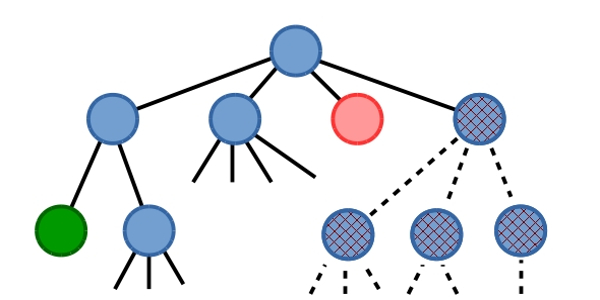
\includegraphics[scale=0.5]{theory_branch_and_bound.jpg}
    \caption{Illustration of the process of solving a CO algorithm with the branch and bound method~\cite{branchimage}.}
\end{figure}

For further information about the most popular strategies or an exhaustive explanation of those techniques, those considered to be good resources are~\cite{fernandes} and~\cite{integeroptimization}.

It is well known that most CO problems can be modeled with mathematical graphs~\citep{appcombinatorial}. Hence, most of the efforts in developing CO algorithms are dedicated to solving graph problems. These efforts have incremented in the last decade on account of the rapid growth in digital technology. Along with this change, the computing needs and the usual assumptions that algorithms used to make have become more demanding in terms of resource allocation.

%% proposals
%% imply
%% thesaurus for synonyms
On one hand, there is a need to research new theoretical proposals and to further investigate the new constraints that modern problems imply. Then, one could use this knowledge to influence the way new strategies approach those problems. On the other hand, there is a pragmatic need to solve those problems in real life and come up with practical and efficient solutions in a considerably small amount of time. In short, the theoretical and practical aspects need to be considered as part of the equation in contemporary applications where strong optimization strategies, like heuristic methods and Integer Programming, are just not enough.

%%%%% Reviewed until here %%%%

The ability to address the underlying issues that emerge in those kinds of problems has been improved drastically during the last years. Those huge steps are directed to obtain fast approximations for CO problems and have given rise to new ways to find algorithms that provide empirically-efficient solutions.

Some recent approaches are being designed to take advantage of Machine Learning capabilities. In particular, Deep Learning strategies are providing alternative ways to deal with some of the underlying issues that arise with those kinds of problems. For specific problems, those approaches have shown to be the most successful in terms of running time efficiency, less human intervention, and the quality of the solutions.

Balanced graph partitioning is one of the fundamental Combinatorial Optimization problems and one which has gotten the best from Deep Learning. Stated in simple words, the Balanced Graph Partitioning Problem is the task of finding a partition of a given graph into mutually exclusive sub-graphs, i.e. they do not share nodes, and the partitions have the same size relative to a given measure. Finding a partition with the desired characteristics is a hard task, but the importance of solving it has incremented in recent years due to its numerous applications.

\section{Objectives}

\subsection{General objective}
    The main target of this research is to develop a machine learning algorithm that solves the graph partitioning problem which is capable of performing on abstract graphs and large-scale graph instances and provide a more robust algorithm.
\subsection{Specific objectives}
The following objectives will help accomplish the general objective:
\begin{itemize}
    \item To understand and analyze the Generalizable Approximate Partitioning (GAP) framework and to use it for solving the graph partitioning problem.
    \item To design an algorithm based on GAP that works for general (non-attributed) graphs and at the same time relies completely on their structure.
    \item To build a framework that is easy to modify in order to use different objective functions in the partitioning stage.
    \item To explore different types of sampling and study the impact they have in the efficiency of the algorithm.
\end{itemize}

\section{Justification}

Graphs are a mathematical representation of what is colloquially known as networks. They are used to describe the relationships between objects and allows one to model an extensive amount of real life problems. Due to their modeling capacity and their power of abstraction, they are widely studied in different areas of computer science and applied mathematics.

The Graph Partitioning (GP) problem is relevant in solving a big number of graph-related tasks. Frequently, GP is employed as a pre-processing subroutine to solve a distinct graph-related problem. If the edges that cross between the partition groups are relatively small compared to the original graph, then the partitioned graph may be more appropriate for analysis and problem-solving than the original~\cite{bettersuited}. 

Finding good-quality partitions of a graph is generally the first step of distributed graph computing tasks. The next paragraphs are dedicated to describe some of the most distinguished applications of GP. Applications of GP to solve graph-related and other abstract computer science problems are presented first followed by some applications to other areas and real-life situations.

One of the first and most useful applications of GP that one can find in literature is graph compression. A popular method for graph compression is the reordering method, which bisects a graph into two sets of equal cardinality aiming to minimize a compression-related objective function. \textit{Graph bisection} is a special case of GP where the objective number of partitions is two. For instance, Bouritsas et. al.~\cite{compressgraphs} showed a way to use a Machine Learning approach combined with a parametric GP algorithm to solve this task.

%%%%% To be completed %%%%
Another important application of GP is to implement \textit{graph sparsification}. Graph sparsification is the task of representin big graphs in a way that takes less space in memory but preserves most of the relevant properties. Spielman and Teng~\cite{sparsification} proposed a novel nearly-linear time partitioning algorithm that is used to produce spectral sparsifiers. The same partitioning algorithm is used by their authors to efficiently solve linear systems~\cite{linearsystems}. In an more recent work, Gatti et. al.~\cite{nesteddissection} presented a way to solve sparse symmetric systems of linear equations using the \textit{nested dissection ordering} algorithm. This algorithm is a divide and conquer heuristic based on GP. Previous work in this algorithms was made by Gupta~\cite{matrixordering}.

Graph partitioning also plays an essential role in paralleling computations and the design of new algorithms on large graphs. For example, in the \textit{device placement} problem one aims to distribute work accross multiple devices. This is a relevant problem in Deep Learning in situations where it is important to train Neural Networks accross multiple devices~\cite{deviceplacement}.

In other applications, Sun et. al. ~\cite{islanding} proposed a solution for the problem "intentional islanding in power systems considering load generation balance" where the main component is GP. For their part, Grady and Schwartz~\cite{imagesegmentation} made use of the isoperimetric constant to generate a GP algorithm that segmentate images.

%%%%%%%%%%%%%%%% End of to be completed %%%%%%%%%%%%%%%%%%

Undoubtedly, the most recent direction where the GP problem has gained importance is in its application for clustering in complex networks. Those types of networks include but are not limited to social networks, transportation networks, web graphs, and biological networks. For an example, see Figure~\ref{fig:complexnetwork}.

\begin{figure}[h!]
    \centering
    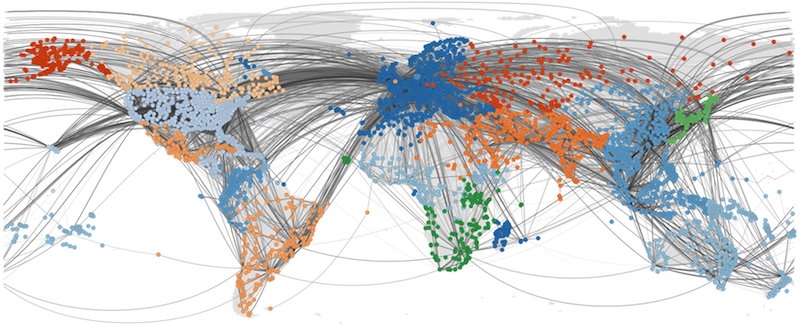
\includegraphics[scale=0.5]{complex_networks.png}
    \caption{The global mobility network. Representation of 4069 airports worldwide where gray lines between them are direct connections \cite{complexnetworks}.}
    \label{fig:complexnetwork}
\end{figure}

An extensive report about the relationship between clustering in complex networks and GP can be found in~\cite{clustering}. That book is a collection of the classical approaches that involves this two related problems. The reader can also look over~\cite{local_clustering} for a more recently-related research.


The approaches followed by most of the mentioned research applications use state-of-the-art GP algorithms. Some of the same algorithms for those tasks are unexplored in modern large-scale graphs, and they do not consider the growth in size of the emerging graph data in the following years. The possibility that they become obsolete in the near future needs to be studied carefully alongside with the development of new strategies that overcome the impending challenges.

Something important to highlight is that the target is not only load-balance but sometimes the minimization of communication volume. This is a consideration not all of the existing approaches have and something worth researching.

%%%%%%%%%%%%% Reviewed until here %%%%%%%%%%

In this context, the project "A Graph Neural Network Approach for Large-Scale Graph Partitioning" was created as a proposal to address some of those challenges. It took one of the most successful algorithms to create ...
that the mentioned applications demand

talk about social relevance and theoretical value.

\section{Project scope and limitations}
During the development of this project the following considerations were taken:
\begin{itemize}
    \item The algorithm has not been tested on real-world graphs. Most of the graphs where the experiments took place were taken from a famous dataset where some of the most successful partitioning algorithms have been tested. Even though this offers a good comparison point, the size of those graphs is pretty small compared to massive graphs like the Amazon or Pinterest networks. The largest graph in the dataset contains $500,000$ nodes.
    \item In general, the graphs used for running the experiments are not dense. However, some of the graphs are dense, but they belong to the category of small-size graphs with less than $50,000$ nodes. Although a number of real-world graphs are sparse, it is suspected that special considerations should be contemplated during the training of the algorithm in the future.
    \item Most of the parameter values are based on previous work where they were shown to have good performance or they were recommended by the original authors. Nonetheless, more experiments in different scenarios should be run to determine better values for the GP specific task.
    \item The machines where the experiments were executed have very limited computing power compared to the ambitions of this project. Though hardware specifications in those machines were enough to run experiments on the dataset, but it would be impossible to process complex networks with this technology.
    \item The proposed algorithm was not designed to run in a distributed environment. Experiments were run in single thread, and the algorithm was trained only in GPU. Modifying the algorithm so it can run in parallel and distributing the training load between the GPU and the CPU are interesting research topics. 
    \item The proposed framework only accepts certain input formats for the graphs, specifically JOSTLE and METIS formats.
    %\item Comparison with GAP was using graphs without features, an interesting thing would be to check performance with the same datasets they used but getting rid of the features, e.g., cora citation
\end{itemize}

\section{Research Problem}
The state-of-the-art algorithms for graph partitioning 
Graph partitioning algorithms based on DL

https://arxiv.org/pdf/2104.03546.pdf
\section{Hypothesis}
When analyzing GAP in depth some observations were made.

\section{Project organization}

The organization of the remaining parts of the thesis is as follows:
\begin{itemize}
    \item In Chapter~\ref{Chapter2}, basic mathematical terminology is presented which is going to be used in the next chapters. Next, this chapter provides a glance at the spectral methods used to solve the GP problem. Then, it finishes with a review of some of the most popular Deep Learning techniques for GP.
    
    \item In Chapter~\ref{Chapter3}, the proposed graph partitioning algorithm for large-scale graphs is presented. It provides a description of the main components in the modules of the framework. Then, it shows how those modules can be used by the algorithm to effectively perform in abstract graphs. Finally, an incorporated sampling technique is used to improve the training process.
    
    \item In Chapter~\ref{Chapter4}, the experiments carried out are described along with the dataset and the comparison metrics used in them. The proposed solution is compared to state-of-the-art methods given the proposed metrics. At the end, the obtained results are summarized.
    
    \item In Chapter~\ref{Conclusion}, a summary of the contributions of this project is given. The advantages of the proposed algorithm over other existing approaches are mentioned as well as further research areas found during its development.
\end{itemize}

